\chapter{Publication II}\label{public_II} 
\textbf{Peer-reviewed publication published in 'Advancing Culture of Living with Landslides'. WLF 2017. Springer International Publishing.}
\vspace{5mm} %5mm vertical space

\textbf{Lima, P.}, Steger, S, Glade, T, Tilch, N, Schwarz, L and Kociu A (2017) Landslide Susceptibility Mapping At National Scale: A First Attempt For Austria, in  Mikos M, Tiwari B, Yin Y, and Sassa K (eds) 'Advancing Culture of Living with Landslides'. WLF 2017. Springer International Publishing, pp. 943 – 951. DOI: 10.1007/978-3-319-53498-5. 

\vspace{5mm} %5mm vertical space

Status of the publication: \textbf{Published.} \textcolor{gray}{Also presented during the 4th World Landslide Forum. Ljubljana, Slovenia, May 29 – June 2, 2017.} \textbf{Link for the program book:} \href{https://wlf4.fgg.uni-lj.si/wp-content/uploads/2017/05/WLF4-Local-Proceedings-and-Programme-with-posters.pdf}{https://wlf4.fgg.uni-lj.si/}\par
\vspace{5mm} %5mm vertical space
\textbf{Link:} \href{https://link.springer.com/chapter/10.1007/978-3-319-53498-5_107}{https://link.springer.com/chapter/10.1007/978-3-319-53498-5_107} \par

\vspace{5mm} %5mm vertical space
This publication suggests a very first attempt to model the Austrian territory through data-driven, statistical modeling. The overall milestone from this publication was to identify potential flawless and weaknesses from large territory modeling using a standard research design. The hypothesis is that most large territories modeling would face similar problems as the Austrian territory did. Once identified, these weaknesses could be then counteracted in future research. Indeed consequences of biased landslide inventories were identified in the outcomes. The corresponding author, \textbf{Pedro Lima} was responsible to write the main parts of this manuscript and do the modeling part. The co-author Stefan Steger, supported intensively these processes, while Thomas Glade contributed with scientific input during the discussion and with feedback on the manuscript. There was also strong collaboration from the Geological Survey of Austria (Nils Tilch, Leonhard Schwarz and Arben Kociu), also offering important input data sets.

%https://tex.stackexchange.com/questions/21248/how-to-add-a-page-number-to-the-included-pdf-pages
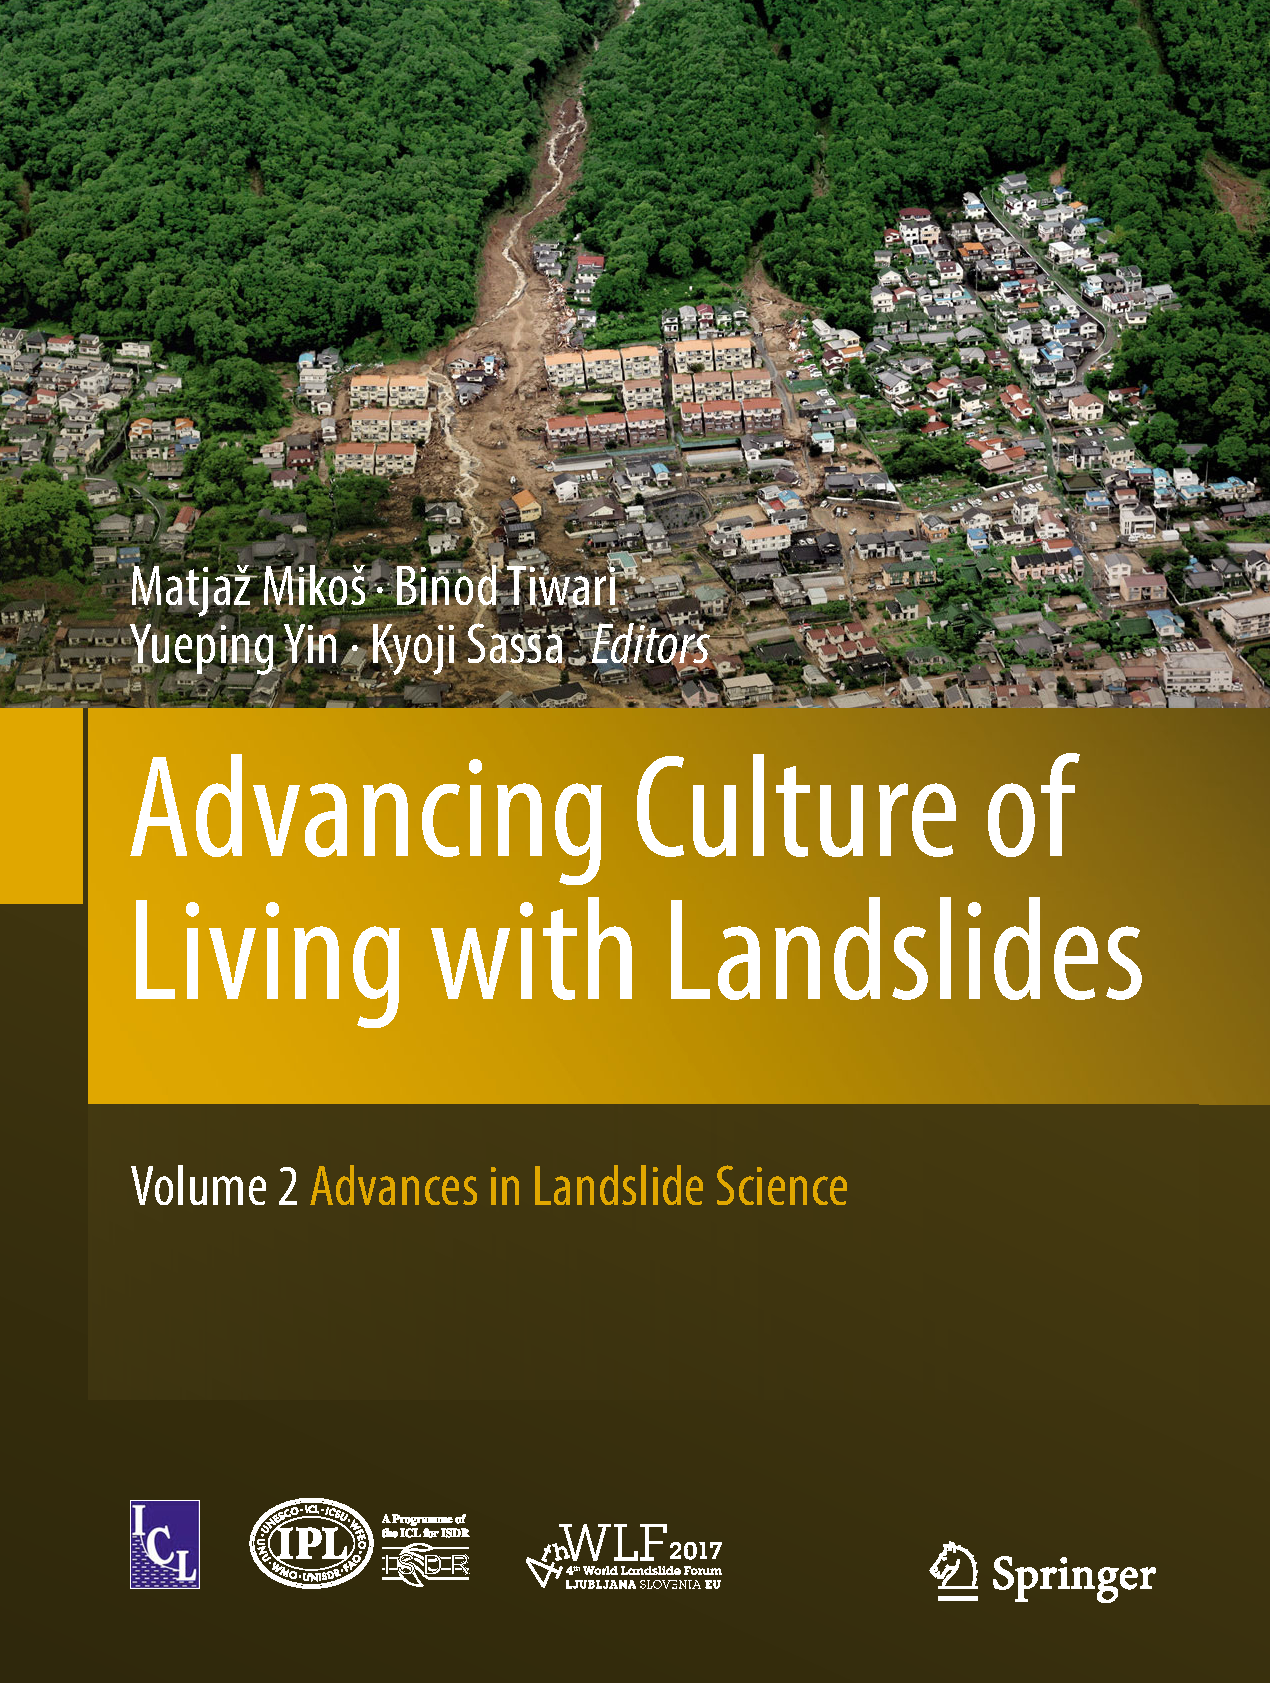
\includepdf[pages=-,scale=0.85, pagecommand={\thispagestyle{plain}}]{figures/PDF/Limaetal2017.pdf}
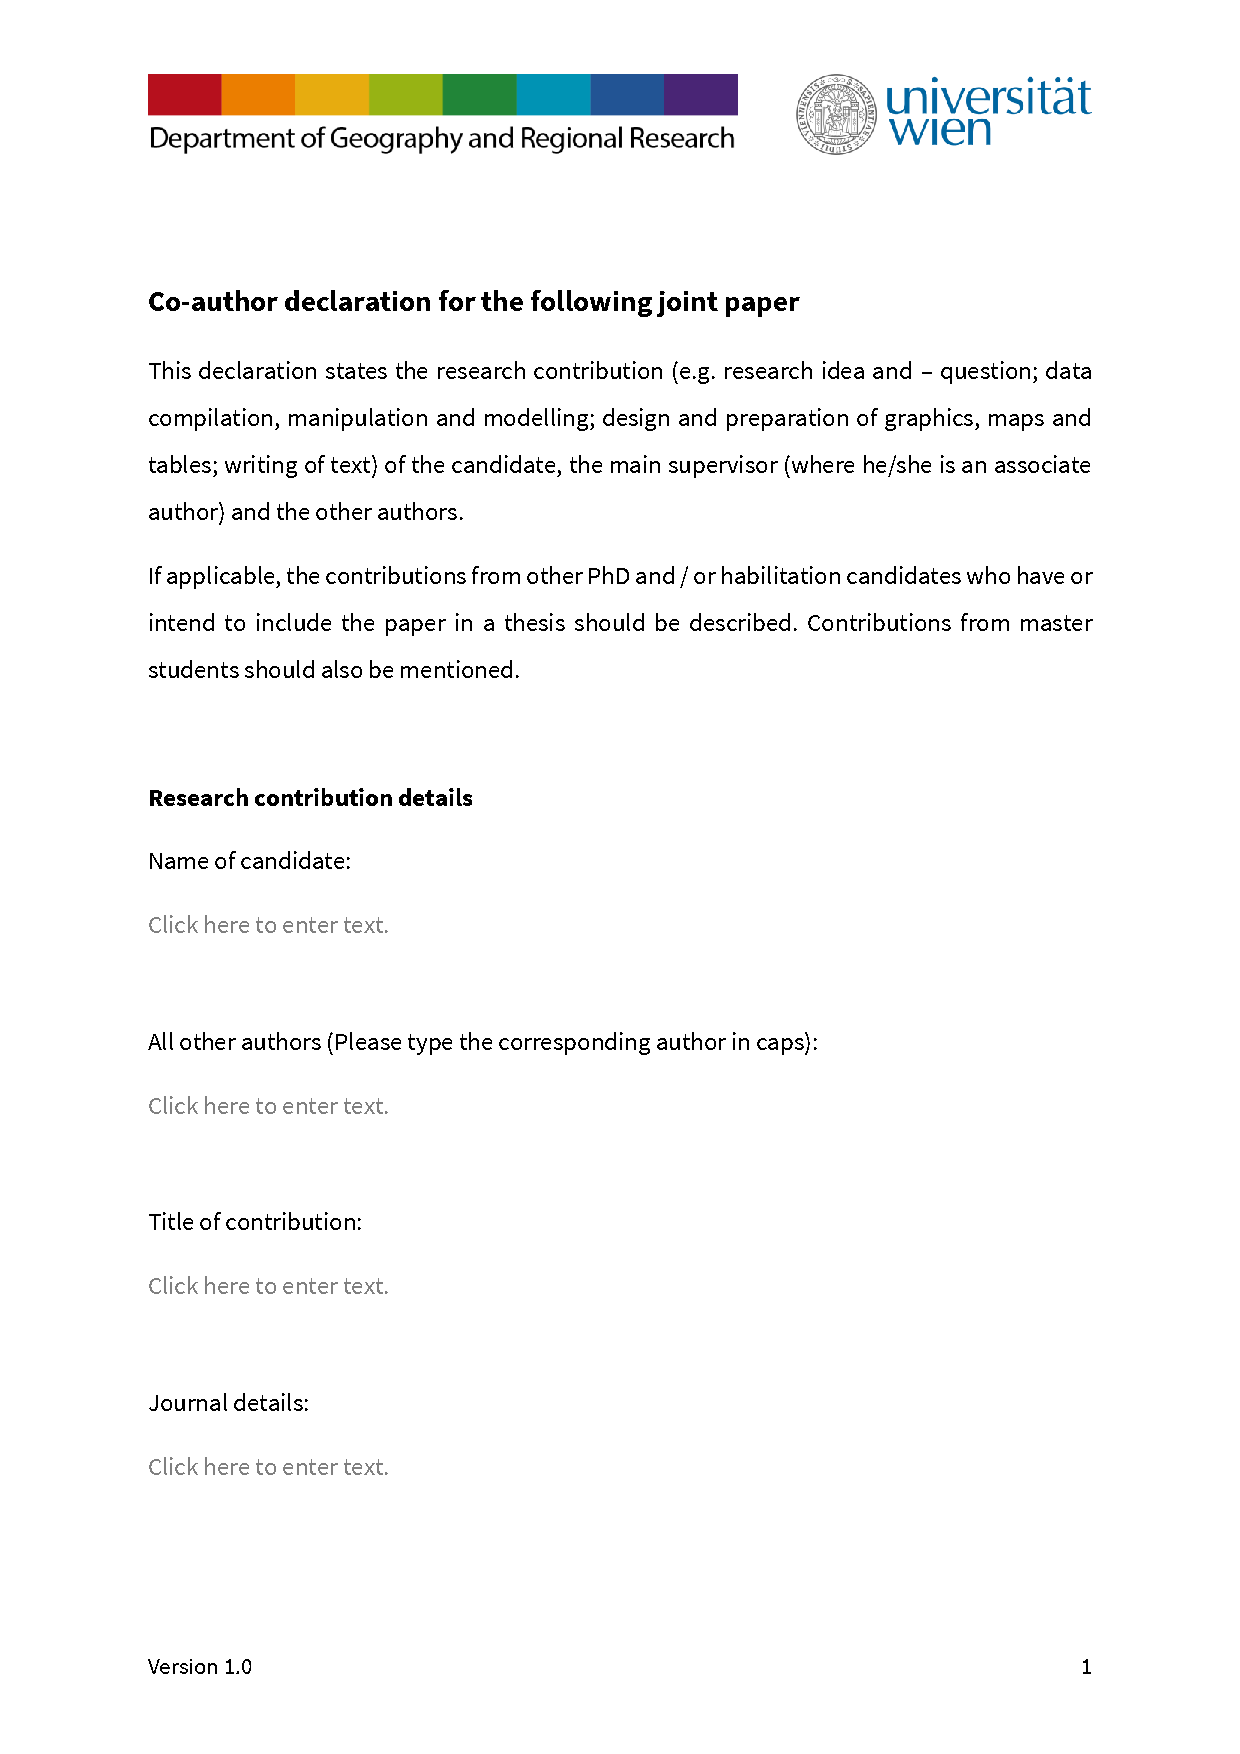
\includepdf[pages=-,nup=1x2,landscape=true]{figures/PDF/co-author_declaration.pdf}
%%%%%%%%%%%%%%%%%%%%%%%%%%%%%%%%%%%%%%%%%%%%%%%%%%%%%%%%%%%%%%%%%%%%%%%%%%%%%%%%%%%%%%%%%%%%%%

